\documentclass[a4paper,12pt]{article}

\usepackage{amsmath,amsfonts,mathtools}
\usepackage{amsthm}
\usepackage{graphicx}
\usepackage{hyperref}
\usepackage{enumitem}

% Personal definitions
\newcommand{\lra}{\ensuremath{\longrightarrow{}}}
\newcommand{\vect}[1]{\mathbf{#1}}
\renewcommand{\qedsymbol}{\rule{0.7em}{0.7em}}

% Theorem commands
\newtheorem{lem}{Lemma}
\newtheorem{thm}{Theorem}
\newtheorem{defn}{Definition}

% Set spacing
\setenumerate{itemsep=1.5pt,parsep=1.5pt,topsep=0.5pt}
\setlist{itemsep=2pt,parsep=1.5pt,leftmargin=1pt}
\setitemize{itemsep=1.5pt,parsep=1.5pt}

% set 1" margins on 8.5" x 11" paper
% top left is measured from 1", 1"
\topmargin       0in
\oddsidemargin   0in
\evensidemargin  0in
\headheight      0in
\headsep         0in
\topskip         0in
\textheight      9in
\textwidth       6.5in

\begin{document}
\title{AlexNet Notes}
\author{Sean Wu}
\date{September 2019}
\maketitle

\tableofcontents

\pagebreak

% set spacing
\setlength{\parindent}{0em}
\setlength{\parskip}{1em}

\section{Intro}

\subsection{Specs}
\begin{itemize}
  \item 60 M params
  \item 650 K neurons
  \item 5 CONV and 3 FC layers
  \item Final 1000-way softmax layer
  \item 5-6 days of training on two GTX 580 3GB GPUs
\end{itemize}

\subsection{Dataset: ImageNet}
\begin{itemize}
  \item ImageNet has $>$ 15 M labelled high res images w/ 22 K categories
  \item AlexNet trained on ILSVRC subset (1000 images in 1000 categories)
  \begin{itemize}
    \item 1.2 M training images
    \item 50 K validation images
    \item 150 K testing images
  \end{itemize}
  \item 2 main KPIs
  \begin{enumerate}
    \item Top-1 error: error rate for most probable label according to model
    \item Top-5 error: fraction of test images for which correct label is not in model's top 5 predictions
  \end{enumerate}
  \item Since ImageNet has variable-res images, images were down-sampled to $256\times 256$
  \begin{itemize}
    \item AlexNet req constant input dimensionality
    \item Images rescaled s.t. shorter side was $L = 256$, then cropped out central $256\times 256$ image from resulting image
  \end{itemize}
\end{itemize}

\section{Architecture}
\subsection{ReLU Nonlinearity}
\begin{description}
  \item[Standard model of neuron output] $f(x) = tanh(x)$ or $f(x) = (1 + e^{-x})^{-1}$ (saturating nonlinearities)
  \item[ReLU] $f(x) = max(0, x)$ (non-saturating nonlinearity)
\end{description}
\begin{itemize}
  \item ReLU units train much faster than $tanh$ units
\end{itemize}

\begin{figure}[t]
  \centering
  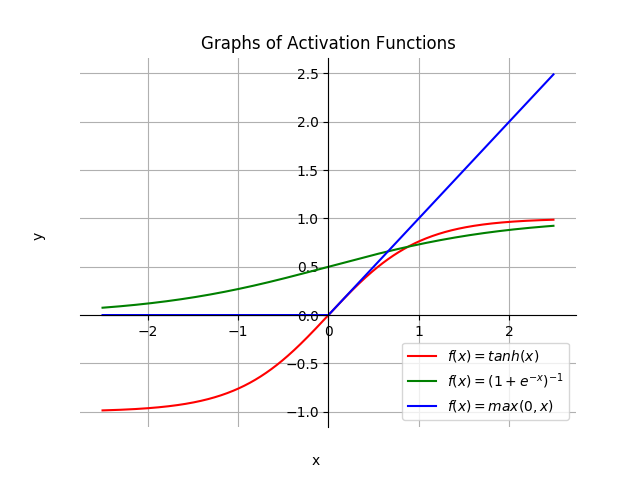
\includegraphics[width=100mm, scale=0.5]{images/ReLU.png}
  \caption{Comparison of ReLU vs other activation functions}
  \label{ReLU}
\end{figure}

\subsection{Multiple GPU Training}
\begin{itemize}
  \item Current GPUs good at cross-GPU parallelization
    \begin{itemize}
      \item Can read/write to another's memory directly w/out going thru host machine memory
    \end{itemize}
  \item AlexNet splits kernels (or neurons) 50/50 across 2 GPUs
  \item AlexNet GPUs only communicate on certain layers which reduces error rates and training time
\end{itemize}

\subsection{Local Response Normalization (Brightness Normalization)}
\begin{itemize}
  \item ReLUs good bec do not req input normalization to prevent saturation
  \item If at least some training examples produce input to a ReLU, learning will happen in that neuron
  \item Adding a local normalization scheme helps generalization
\end{itemize}
\begin{description}
  \item[Response-normalized activity $b^i_{x,y}$] is given by:
  \begin{equation}
    b^i_{x,y} = a^i_{x,y}/\left(k + \alpha\sum^{min(N-1,i+n/2)}_{j=max(0,1-n/2)}(a^j_{x,y})^2\right)^\beta
  \end{equation}
  where $a^i_{x,y}$ is activity of a neuron computed by applying kernel $i$ at position $(x,y)$ and then applying ReLU nonlinearity and $N$ is total number of kernels in layer. The sum runs over $n$ "adjacent" kernel maps at same spatial position,
\end{description}
\begin{itemize}
  \item Constants $k$, $n$, $\alpha$, and $\beta$ are hyperparameters determined using validation set
\end{itemize}

\subsection{Overlapping Pooling}
\begin{itemize}
  \item Pooling layers in CNNs summarize outputs of groups of neurons in same kernel map
  \item Pool layer like grid of pooling units spaced $s$ units apart, each summarizing a $z\times z$ neighborhood centered at location of unit
  \begin{enumerate}
    \item if $s = z$: traditional local pooling
    \item if $s < z$: overlapping pooling
  \end{enumerate}
  \item AlexNet uses overlapping pooling w/ $s = 2$ and $z = 3$
  \begin{itemize}
    \item Slightly reduced error and harder to overfit
  \end{itemize}
\end{itemize}

\subsection{Layers Architecture}
\begin{itemize}
  \item INPUT \lra CONV \lra 3 FC \lra 1000-way softmax
  \item Maximizes multinomial logistic regression objective
  \begin{itemize}
    \item Equivalent to maximizing average across training cases of log-probability of correct label under prediction distribution
  \end{itemize}
  \item Kernels of 2nd, 4th, 5th CONV layers only connected to kernel maps in prev layer on same GPU
  \begin{itemize}
    \item Kernels in 3rd GPU fully connected to all kernel maps in 2nd layer
  \end{itemize}
  \item Response-normalization follow 1st and 2nd CONV layers
  \begin{itemize}
    \item 3rd, 4th, 5th layers connected w/ no pooling or normalization layers
  \end{itemize}
  \item Max pooling follow both response-normalization and 5th CONV
  \item ReLU non-linearity applied to output of all CONV and FC
\end{itemize}

\pagebreak

\subsubsection{Diagrams of AlexNet Layers}

\begin{figure}[htp]
  \centering
  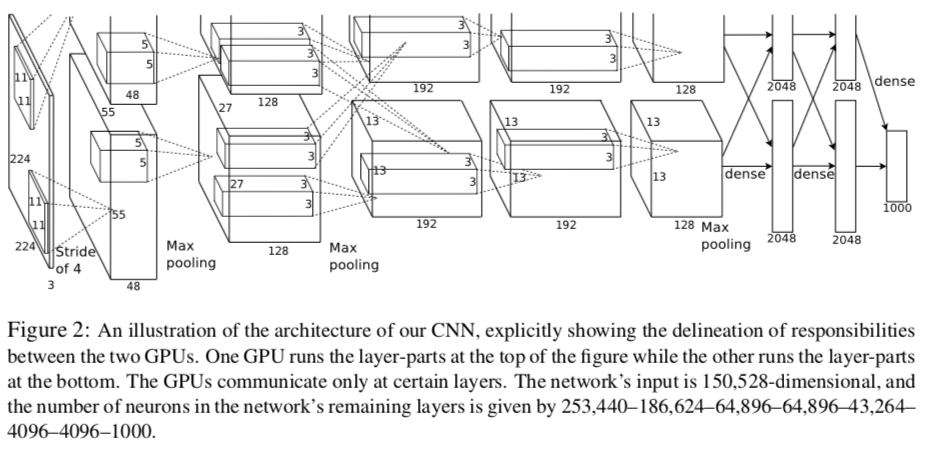
\includegraphics[width=140mm, scale=0.75]{images/AlexNet-GPU-Structure.png}
  \caption{Diagram showing AlexNet layers split by GPU}
  \label{AlexNet-Struct}
\end{figure}

\begin{figure}[htp]
  \centering
  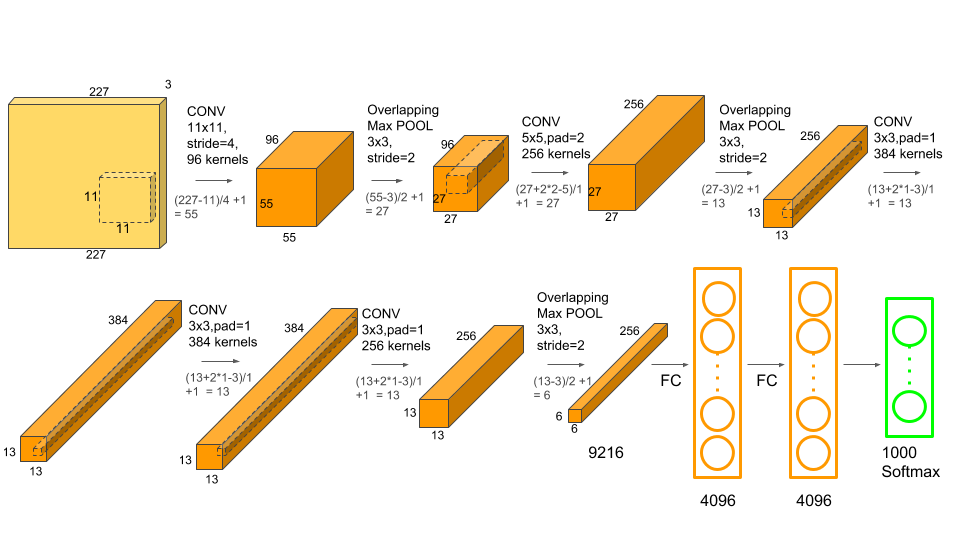
\includegraphics[width=140mm, scale=0.75]{images/AlexNet-1.png}
  \caption{Diagram showing AlexNet layers with filter sizes and strides}
  \label{AlexNet-Layers}
\end{figure}

\pagebreak

\section{Reducing Overfitting}
\subsection{Data Augmentation}
\begin{itemize}
  \item Artificially enlarged dataset w/2 forms of label-preserving transformations
  \item Transformed images generated on CPU while GPU training on previous set of training images
  \begin{itemize}
    \item No need to store transformed images
    \item Effectively computationally free
  \end{itemize}
\end{itemize}

\subsection{Data Augmentation Methods}
\begin{enumerate}
  \item Image translations and reflections
  \begin{itemize}
    \item Extract random $224\times 224$ patches (sometimes horizontal reflected) from $256\times 256$ images and train on extracted patches
    \item Increases training set size by factor of 2048, but resulting traning examples are very interdependent
    \item At test time, network makes prediction by selecting 10 patches (4 corners + 1 centre + 5 reflections) and averaging predictions on patches using softmax
  \end{itemize}
  \item Altering RGB channel intensities
  \begin{itemize}
    \item Perform PCA (principal component analysis) on set of RGB pixel values
    \item Add multiples of principal components w/ magnitudes proportional to corresponding eigenvalues times a random var from Gaussian w/ mean 0 and standard dev 0.1
    \item Thus for each RGB image pixel $I_{xy} = \begin{bmatrix}I^R_{xy}, I^G_{xy}, I^B_{xy}\end{bmatrix}^T$, add:
    \begin{equation}
      \begin{bmatrix}
        \vect{p_1}, \vect{p_2}, \vect{p_3}
      \end{bmatrix}
      \begin{bmatrix}
        \alpha_1\lambda_1, \alpha_2\lambda_2, \alpha_3\lambda_3
      \end{bmatrix}^T
    \end{equation}
  \end{itemize}
\end{enumerate}
where $\vect{p_i}$ and $\lambda_{i}$ are the $i$th eigenvector and eigenvalue of the $3\times 3$ covariance matrix of RGB pixel values and $\alpha_i$ is the random variable
\begin{itemize}
  \item Transformation works because object identity is invariant to changes in intensity and color of illumination
\end{itemize}

\subsection{Dropout}
\begin{itemize}
  \item Can reduce test errors by combining predictions of different models, but very time expensive
\end{itemize}
\begin{description}
  \item[Dropout] zeroing output of each hidden neuron w/ probability 0.5
\end{description}
\begin{itemize}
  \item Very efficient model combination method, but doubles \# of iterations req to converge
  \item Dropped out neurons do not contribute to forward pass or backpropagation
  \item For every new input, neural net samples a different architecture, but all architectures share weights
  \item Reduces complex co-adaptations of neurons since a neuron cannot rely on presence of particular neurons
  \begin{itemize}
    \item Neurons force to learn more robust features that are useful in conjunction w/ other random subsets of neurons
  \end{itemize}
  \item At test time, use all neurons but multiply outputs by 0.5 (approximation of taking geometric mean of predictive distributions produced by exponentially many dropout networks)
  \item Use dropout in first 2 FC
\end{itemize}

\section{Details of Learning}
\begin{itemize}
  \item AlexNet trained using gradient descent w/ batch size of 128, momentum of 0.9, and weight decay of 0.0005
  \begin{itemize}
    \item Small weight decay reduces training error
  \end{itemize}
  \item Weights initialized from zero-mean Gaussian distribution w/ standard deviation of 0.01
  \item Update rule for weight $w$ was:
\end{itemize}
\begin{align}
  v_{i+1} &\coloneqq 0.9\cdot v_i - 0.0005\cdot\epsilon\cdot w_i - \epsilon\cdot \biggl\langle\frac{\partial L}{\partial w}\Bigl|_{w_i} \biggr\rangle_{D_i} \\
  w_{i+1} &\coloneqq w_i + v_{i+1}
\end{align}
where $i$ is the iteration index, $v$ is the momentum, $\epsilon$ is the learning rate, and $\Bigl\langle\frac{\partial L}{\partial w}\Bigl|_{w_i} \Bigr\rangle_{D_i}$ is the average over the $i$th batch $D_i$ of the derivative of the objective wrt $w$, evaluated at $w_i$
\begin{itemize}
  \item Neuron biases in 2nd, 4th, and 5th layers \& FC layers initialized w/ constant 1
  \begin{itemize}
    \item This initialization speeds up early learning stages by providing ReLUs w/ positive input
  \end{itemize}
  \item Neuron biases in other layers initialized w/ constant 0
  \item Used equal learning rate for all layers, and adjusted manually through training
  \item Adjustment heuristic: divide learning rate by 10 when validation error stopped improving
  \item Learning rate initialized at 0.01 and reduced 3 times before termination
\end{itemize}


\end{document}
